\subsection{Traditional Harmony Search and some variants}
\subsubsection{Harmony Search Metaheuristic}
is a population-based metaheuristic algorithm inspired from the musical process of searching for a perfect state of Harmony or Aesthetic Quality of a Harmony (AQH). The HS was proposed by Z. W. Geem et al.\cite{DBLP:journals/simulation/GeemKL01}. In other words, the main idea of the HS metaheuristic is to mimic the process performed by musicians when they try to play a beautiful harmony.

For the purpose of properly understand what is looking like a good solution in this metaheuristic, we must know the meaning of AQH. The AQH in an instrument is essentially determined by its pitch (or frequency), sound quality, and amplitude (or loudness). The sound quality is mainly determined by the harmonic content that is in turn, determined by the waveforms or modulations of the sound signal. However, the harmonics that it can generate will largely depend on the pitch or frequency range of the particular instrument \cite{Geem:2009:MHS:1643438}. Different notes have different frequencies. For example, the note A  has a fundamental frequency $f_0=440 Hz$. The fundamental frequency of each note can be seen in (Table~\ref{fig:musical_notes}). 

\begin{table}[H]
\centering
\begin{tabular}{|l|l|}
\hline
\textbf{Musical Note} & \textbf{Frequency} \\ \hline
C                     & 261,625565 Hz      \\ \hline
D                     & 293,664768 Hz      \\ \hline
E                     & 329,627557 Hz      \\ \hline
F                     & 349,228231 Hz      \\ \hline
G                     & 391,995436 Hz      \\ \hline
A                     & 440,000000 Hz      \\ \hline
B                     & 493,883301 Hz      \\ \hline
\end{tabular}
\caption{HS - Musical Notes}\label{fig:musical_notes}
\end{table}

Given the above, it is established that a good harmony has good AQH. The pitch of each musical instrument determines the AQH, just as the fitness function values determines the quality of solution.

In the music improvisation process, all musicians (Table~\ref{fig:harmony_process_musician}) sound pitches (Table~\ref{fig:harmony_process_pitch_range}) within possible range together to make one harmony (Table \ref{fig:harmony_process_solution}), If all pitches make a good harmony, each musician stores in his memory that experience and possibility of making a good harmony (Table \ref{fig:harmony_process_aesthetics}) in increased next time. The same thing in optimization: the initial solution is generated randomly from decision variables within the possible range, If the objetive function values of these decision variables is good to make promising solution, then the possibility to make a good solution is increased next time.

In this document, the researcher set its focus on studying the classical SCP problem, given by equation \eqref{ec:set-covering-1}, where we want minimize the cost of solution.\\

The traditional HS metaheuristic has five steps \cite{DBLP:journals/asc/ZouGLW11}, which will be reviewed below.

%MUSICOS (musician - > decision variables)
\squeezeup
\begin{table}[!h]
\centering
\begin{tabular}{|m{1.5cm}|m{8cm}|}
\hline
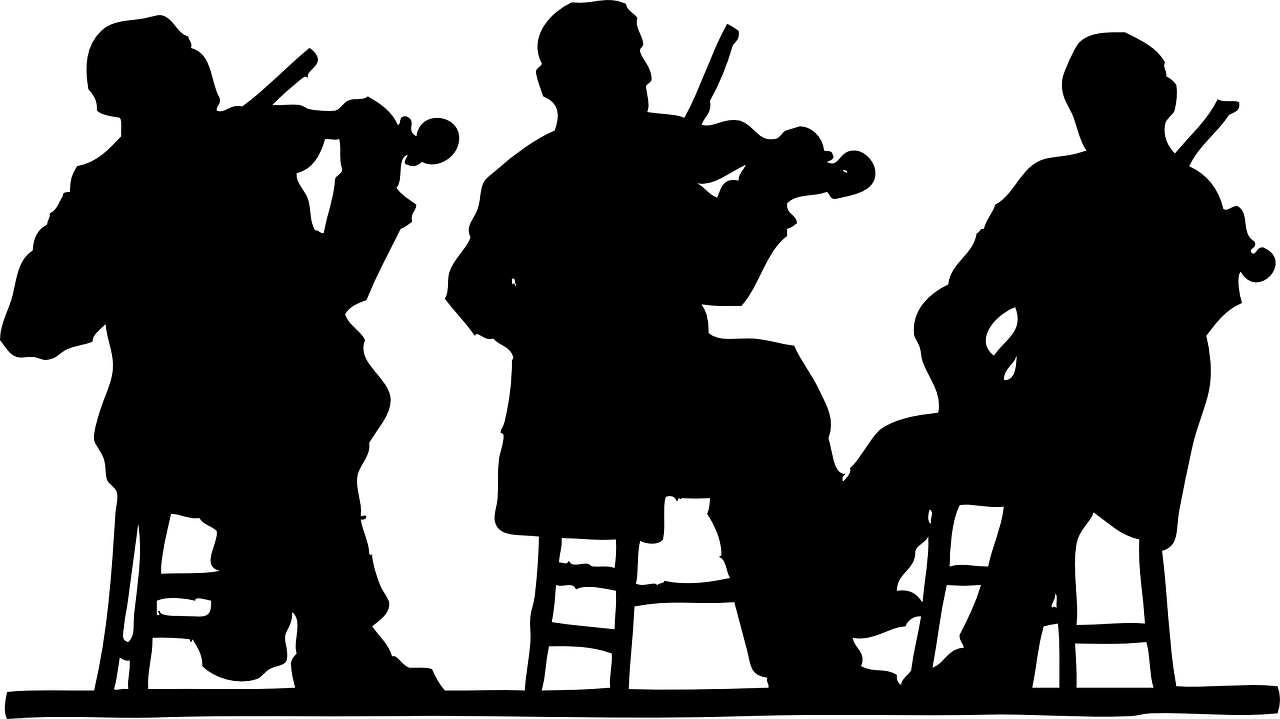
\includegraphics[width=15mm,scale=0.05]{MarcoTeorico/imagenes/musicos.png} & 
Each musician represents a decision variable,
according to the example shown, there would be 11 musicians, 	
since there are 11 decision variables $x_1\dots x_{11}$. \\ \hline
\end{tabular}
\caption{HS components - Musician}\label{fig:harmony_process_musician}
\end{table}
\squeezeup

%--VIOLIN (Instrument Pitch Range - > Range Value of decision variable)
\squeezeup
\begin{table}[!h]
\centering
\begin{tabular}{|m{1.5cm}|m{8cm}|}
\hline
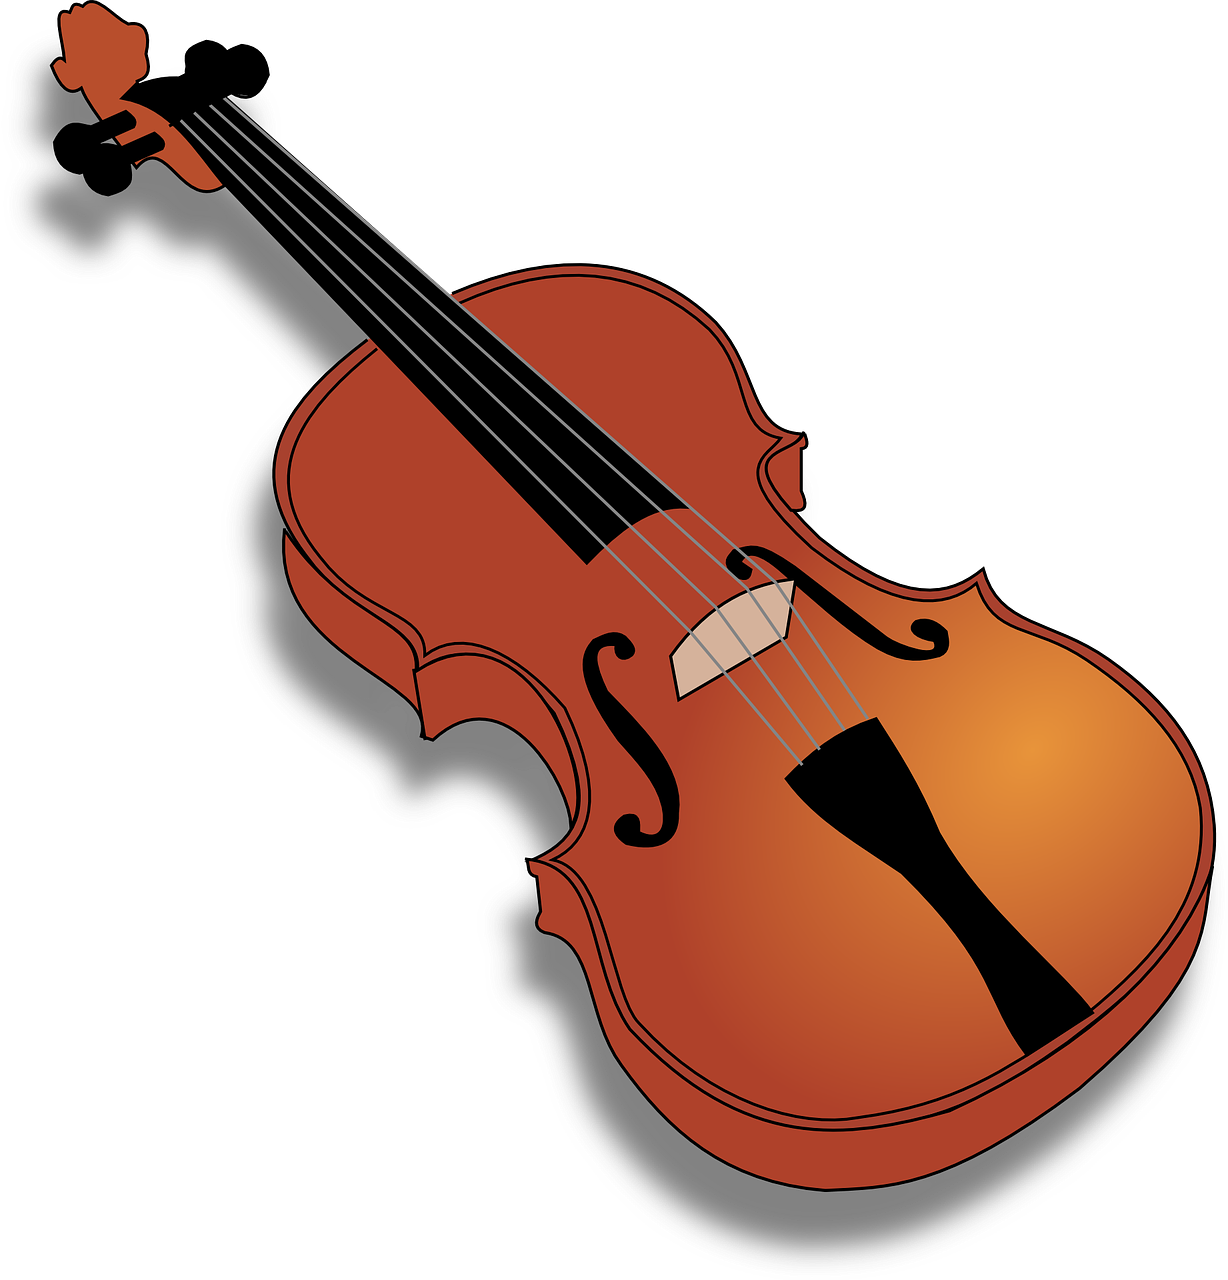
\includegraphics[width=10mm,scale=0.02]{MarcoTeorico/imagenes/violin.png} & The pitch range of the instrument represents the range of values that can take a decision variable. Given the nature of the SCP, the possible values are ${\{0,1\}}$ \\  \hline\end{tabular}
\caption{HS components - Pitch range}\label{fig:harmony_process_pitch_range}
\end{table}
\squeezeup


%--NOTA MUSICAL (Armonia -> Solucion)
\squeezeup
\begin{table}[!h]
\centering
\begin{tabular}{|m{1.5cm}|m{8cm}|}
\hline

\includegraphics[width=10mm,scale=0.0005]{MarcoTeorico/imagenes/nota.png} & Musical harmony at a certain time, corresponds to a solution at a certain iteration.\\ \hline
\end{tabular}
\caption{HS components - Solution}\label{fig:harmony_process_solution}
\end{table}
\squeezeup
% CALIDAD ESTETICA (Calidad de la armonia -> Calidad de la soluci�n)
\squeezeup
\begin{table}[!h]
\centering
\begin{tabular}{|m{1.5cm}|m{8cm}|}
\hline

\includegraphics[width=15mm,scale=0.02]{MarcoTeorico/imagenes/audience.png} & Aesthetics audience, judges whether harmony is good or not.� In the problem it refers to the objective function.\\ \hline
\end{tabular}
\caption{HS components - Aesthetics audience}\label{fig:harmony_process_aesthetics}
\end{table}
\squeezeup
%FIN TABLAS

\textbf{Step 1:  Initialize the problem and algorithm parameters.} \\
The optimization problem is defined as shown in equation \eqref{ec:set-covering-1} where the goal is to minimize $Z$ subjec to equations \eqref{ec:set-covering-2} and \eqref{ec:set-covering-3}. $x_{iL}$ and $x_{iU}$ are the lower and upper bounds for decision variables. The required parameters to solve the optimization problem, that is, Harmony Memory Size (HMS) or number of solution vectors in the harmony memory, Harmony Memory Consideration Rate (HMCR) which determines the rate of selecting the value from the memory and Pitch Adjusting Rate (PAR) which determines the probability of local improvement and number of improvisations ($NI$) are given when the metaheuristic begins.\\

\textbf{Step 2: Initialize the harmony memory.} \\
 An initial HM is filled with a population of  Harmony Memory Size (HMS). We can formally say the following: $x_i^j = x_{iL} + rand()(x_{iU} - x_{iL}), ~ j=1,2, \ldots , HMS$. Where rand() is a random from a uniform distribution of $[0,1]$.\\
 
\textbf{Step 3:  Improvise a new harmony.} \\
Harmonies are generated randomly and the details of the procedure to improvise harmony $x_i^{ \ensuremath{'}}$ can be given in Algorithm \ref{alg:impr_new_harmony}. According to the process, vectors are generated as follows $(x^1,\ldots,x^{HMS})$. Vectors results , make up a matrix such as that shown in (Figure~\ref{mat:sol_mat}):
 
 \begin{figure}
 $$
HM=
 \begin{bmatrix}
x_1^1 & \ldots & x_n^{1}\\ 
\vdots & \ddots & \vdots \\ 
x_1^{HMS} & \ldots  & x_n^{HMS}
\end{bmatrix}
$$
\caption{Harmony Memory Matrix}\label{mat:sol_mat}
\end{figure}

%ALGORITMO DE IMPROVISACION _____________________________
\squeezeup
\begin{algorithm}
      \For{$i\leftarrow 1$ \KwTo $n$}{    	
	\eIf{rand()$\leq$HMCR}
      	{
		$x_i^{ \ensuremath{'}}$ = $x_i^j$~($j=1,2,\ldots,$HMS) \mbox{//memory consideration}\\
		\lIf{rand() $\leq$ PAR} {
			$x_i^{\ensuremath{'}}$ = $x_i^{ \ensuremath{'}} \pm r(bw)$ \mbox{bw is the amount of maximum change in pitch adjustment}
      		}
      	}
      	{
        		$x_i^{ \ensuremath{'}}$ = $x_{iL}$ + rand() $(x_{iU} - x_{iL})$ \mbox{//random selection}
      	}
      }
    \caption{Generating new harmony for traditional HS}\label{alg:impr_new_harmony}
\end{algorithm}
\squeezeup
%__________________________________________________________

\textbf{Step 4: Update harmony memory.} \\
If the new generated harmony $x^{\ensuremath{'}}$ = ($x_{1}^{\ensuremath{'}}$, $x_{2}^{\ensuremath{'}}$ , \ldots,~$x_{n}^{\ensuremath{'}} $) has a better fitness than the worst one $x_{worst}$ in HM, then replace the worst harmony with the new one $x_{worst} \leftarrow x^{\ensuremath{'}}$; otherwise , go to the next step. \\

\textbf{Step 5: Check the stop criteria.} \\
If the stopping criterion (e.g. maximum number of iterations $NI$) is satisfied, computation is
terminated. Otherwise, step 3 is repeated.\\


\subsubsection{Global-Best Harmony Search Metaheuristic}
To further improve the convergence performance of HS and overcome some shortcomings of HS, a new variant of HS, called  Global-Best Harmony Search (GHS), was proposed by Omran and Mahdavi \cite{DBLP:journals/amc/OmranM08}. 
First, the GHS dynamically updates parameter PAR according to equation (\ref{ec:PAR-T}):

\begin{equation} \label{ec:PAR-T}
PAR(t) = PAR_{min}+\frac{PAR_{max} - PAR_{min}}{NI}t
\end{equation}

where $PAR(t)$ represents the pitch adjusting rate at generation $t$, $PAR_{min}$ and $PAR_{max}$  are the minimum and maximum adjusting rate, respectively.
The parameter $t$ is the iterative variable, and parameter $NI$ is the number of improvisations.

\subsubsection{Binary Global-Best Harmony Search Metaheuristic}

The HS is good at identifying the high performance regions of the solution space in a reasonable time, but poor at performing local search \cite{DBLP:journals/eswa/XiangALHZ14}. Namely, there is an unbalance between the exploration and the exploitation of HS. Furthermore, HS designed for continuous space cannot be directly used to solve discrete combinatorial optimization problems.

In order to overcome the drawbacks of HS, a novel binary global-best harmony search (BGBHS) is designed for binary optimization problems.

%Owing to better performance of GHS, some modifications are introduced to further enhance the convergence performance. Then a novel binary, a two-phase repair operator \ref{alg:addAndDrop}, and a greedy selection mechanism are integrated into the BGHS, and they are described in detail as follows.

%------------------------------Diagrama de HS
\begin{figure}[H]
\centering
\begin{tikzpicture}[align = flush center, font = \small, node distance = 12mm, scale=0.6, every node/.style={scale=0.6}] %[node distance = 15mm, auto]
\node (start) [startstop] {Start};
\node (pro1) [process, below of=start] {Initialize parameters};
\node (pro2) [process, below of=pro1] {Initialize Harmony Memory (HM)};
\node (pro3) [process, below of=pro2] {Repair all harmonies in HM};
\node (pro4) [process, below of=pro3] {$t=1$};
\node (pro5) [process, below of=pro4] {Save $x_{best}$ and $x_{worst}$ harmony};
\node (proB) [process, below of=pro5]{$x_{new} = $ Bernoulli trial \smallskip $\forall {x_{new}}_j \in \{0,1\}$, and $j=\{1 \dots n\}$};
\node (pro6) [process, below of=proB] {Rand() $\leq$ HMCR};
\node (pro7) [process, below of=pro6] {Rand() $\leq$ PAR};
\node (pro8) [decision, below of=pro7] {$j < n$};
\node (pro9) [process, left of=pro8, xshift=-1.5cm] {$j = j + 1$};
\node (pro10) [decision, below of=pro8, yshift=-0.2cm] {$x_{new}$ is better than $x_{best}$};
\node (pro11) [process, right of=pro10, xshift=4.0cm] {$x_{best} = x_{new}$};
\node (pro12) [decision, below of=pro10, yshift=-1.0cm] {$x_{new}$ is better than $x_{worst}$};
\node (pro13) [process, right of=pro12, xshift=2.5cm] {$x_{worst} = x_{new}$};
\node (pro14) [decision, below of=pro12, yshift=-1.0cm] {Termination criterion is met?};
\node (pro15) [process, left of=pro14, xshift=-3.5cm] {$t=t+1$};
\node (pro16) [process, below of=pro14, yshift=-0.8cm] {Output Result};

%---------------------------------ARROWS
\draw [arrow] (start) -- (pro1);
\draw [arrow] (pro1) -- (pro2);
\draw [arrow] (pro2) -- (pro3);
\draw [arrow] (pro3) -- (pro4);
\draw [arrow] (pro4) -- (pro5);
\draw [arrow] (pro5) -- (proB);
\draw [arrow] (proB) -- (pro6);
\draw [arrow] (pro6) -- (pro7);
\draw [arrow] (pro7) -- (pro8);
\draw [arrow] (pro8) -- (pro9) node [midway, above] {Y};
\draw [arrow] (pro9) |- (pro6);
\draw [arrow] (pro8) -- (pro10) node [midway, left] {N};
\draw [arrow] (pro10) -- (pro11) node [midway, above] {Y};
\draw [arrow] (pro10) -- (pro12) node [midway, left] {N};
\draw [arrow] (pro12) -- (pro13) node [midway, above] {Y};
\draw [arrow] (pro12) -- (pro14) node [midway, left] {N};
\draw [arrow] (pro14) -- (pro15) node [midway, above] {N};
\draw [arrow] (pro15) |- (pro5);
\draw [arrow] (pro11) |- (pro14) ;
\draw [arrow] (pro13) |- (pro14) ;
\draw [arrow] (pro14) -- (pro16) ;

\end{tikzpicture}
\caption{The flowchart of BGBHS algorithm.}\label{dia:Asdsd}
\end{figure}

%------------------------------nueva_armonia_agresiva():

\begin{algorithm}

\SetKwProg{Fn}{Function}{}{}
\Fn{new_aggressive_harmony ()}{
 CostVector $\gets$ getCostVector()\\
 ProfitVector $\gets$ getMu_j(CostVector)\\
 AMatrix $\gets$ getAMatrix()\\
\ForEach{row in AMatrix}{
	RowCost $\gets$ row * ProfitVector
	LowCost $\gets$ getMaxValue(ProfitVector)
	
}
 

}

    \caption{Generating a new greedy harmony}\label{alg:newHarmonyGreedy}
\end{algorithm}

%------------------------------Fase ADD y DROP:
\begin{algorithm}
\begin{algorithmic}[1]
 \STATE //ADD Phase
\STATE $M \gets 1,2,\ldots, m$
\STATE $A_i \sum_{j=1}^{n} a_{ij}x_{j}, i \in M$
\FOR{$j \gets 1$ \TO $n$} {
	\IF{$x_j = 0$ and $\exists i \in M, A_i < 1$ } {
		\STATE $x_j \gets 1$
		\STATE $A_i \gets A_i + a_{ij}$
	}\ENDIF
} \ENDFOR

\STATE //DROP Phase
\FOR{$j \gets n$ \TO $1$}{
	\IF{$x_j = 1$ and $\exists i \in M, A_i - a_{ij} \geq 1$ } {
		\STATE $x_j \gets 0$
		\STATE $A_i \gets A_i - a_{ij}$
	}\ENDIF
} \ENDFOR

\caption{Repair operator ADD and DROP}\label{alg:addAndDrop}
\end{algorithmic}
\end{algorithm}













